\begin{figure}[h]
  \begin{center}
    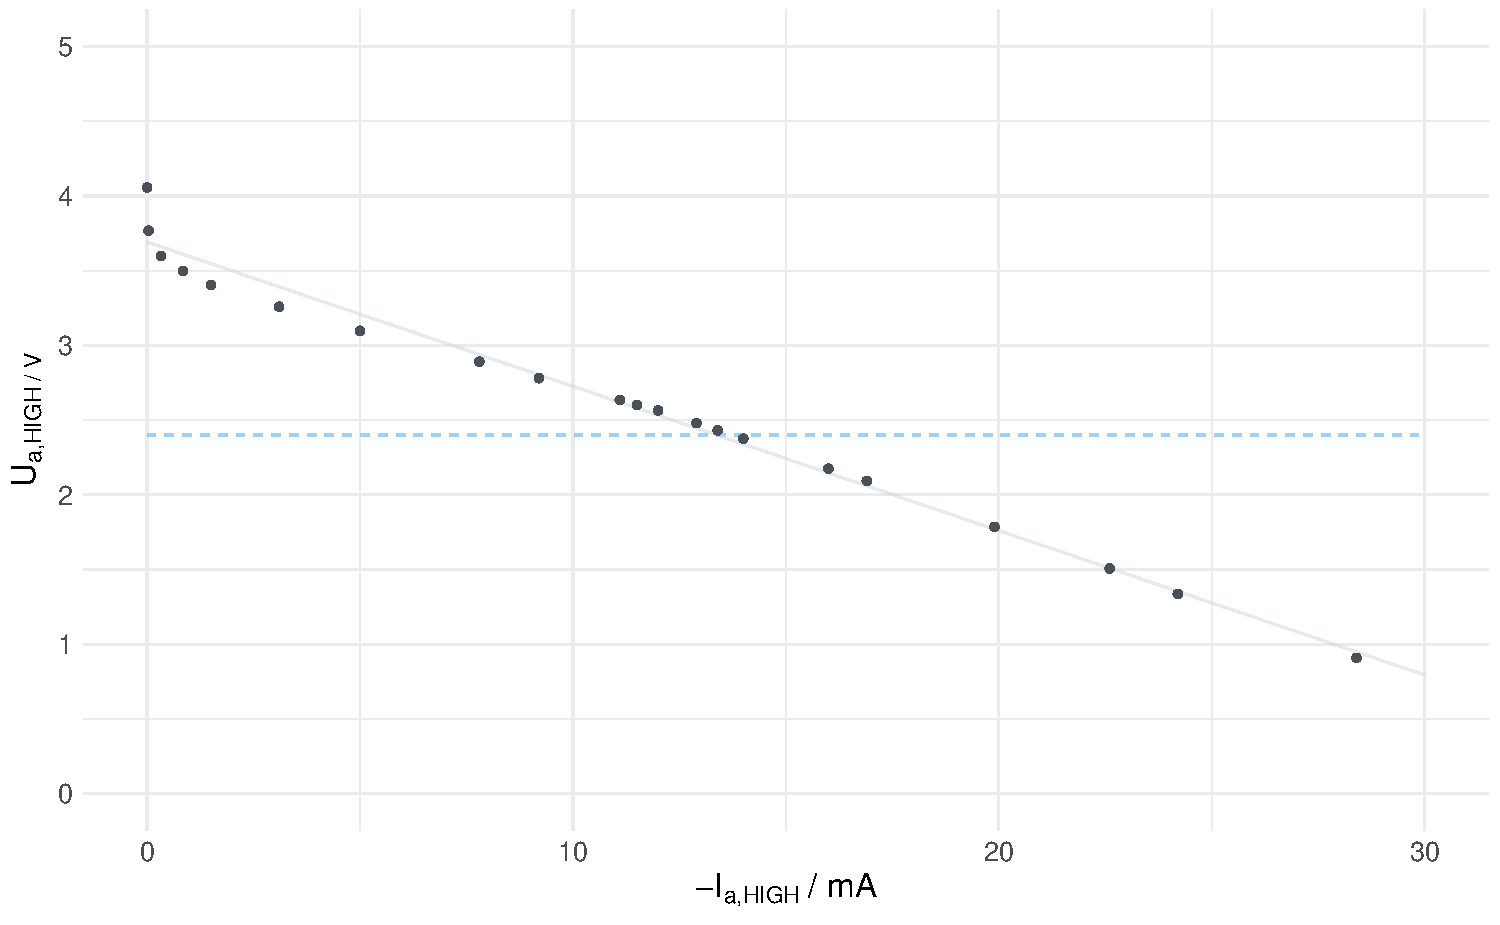
\includegraphics[width=\textwidth]{VERA/SN7400/SN7400_Ausgangskennlinie_high}
  \end{center}
  \caption{Graph der Messwerte von Ausgangs-HIGH-Strom und -Spannung, die blaue
    Linie stellt die TTL-HIGH-Grenze dar}
  \label{fig:aus_schnib_high}
\end{figure}

Der Lastwiderstand am Gatterausgang wurde bei HIGH-Pegel mit einer
Widerstandsdekade verändert. Dadurch konnte die Ausgangs-HIGH-Spannung des
Gatters bei Variation des Ausgangs-HIGH-Stromes ermittelt werden.


Auch hier
ergibt sich ein recht linearer Zusammenhang zwischen Strom und Spannung, welcher
in einer Änderungsrate von etwa $- 96.64 \, \si{\milli\volt}$ Ausgangsspannung
je $1 \, \si{\milli\ampere}$ Ausgangsstrom resultiert (betragsmäßig), was einem
statischen Widerstand von $96.64 \, \Omega$ ($U_\mathrm{a,HIGH}(0) = 3.6926 \,
\si{\volt}$) entspricht (Abb. \ref{fig:aus_schnib_high}).

Man kann sehen, dass bei einem Strom von etwa $-16
\,\si{\milli\ampere}$ die TTL-Schwelle für die genaue Erkennung des
Ausgangsspannungspegels als HIGH unterschritten wird und der Pegel mit
steigendem Ausgangsstrom immer weiter in den undefinierten Bereich fällt, in welchem
keine zuverlässige Funktion folgender Gatter gewährleistet werden kann.

\begin{table}[h]
    \centering
\begin{minipage}[t]{0.48\linewidth}\centering

    \begin{tabular}{ll}
      \rowcolor{gray0} 
      $I_\mathrm{a, LOW}$ & $U_\mathrm{a, LOW}$ \\
      15.8                & 0.1814              \\
      14.8                & 0.175               \\
      13                  & 0.164               \\
      12                  & 0.1572              \\
      10.9                & 0.1496              \\
      10                  & 0.1433              \\
      8.9                 & 0.1357              \\
      8.1                 & 0.1306              \\
      7                   & 0.1222              \\
      6                   & 0.1146              \\
      5.1                 & 0.1082              \\
      4                   & 0.0987              \\
      3                   & 0.0904              \\
      2                   & 0.0806              \\
      1.02                & 0.0704              \\
      0.503               & 0.0645              \\
      0.247               & 0.0614              \\
      0.123               & 0.0599             
    \end{tabular}
  \caption{Messwerte der Ausgangs-LOW-Spannung in Abhängigkeit vom Ausgangs-LOW-Strom}
  \label{tab:aus_low}

\end{minipage}\hfill%
\begin{minipage}[t]{0.48\linewidth}\centering

    \begin{tabular}{ll}
      \rowcolor{gray0} 
      $I_\mathrm{a, HIGH}$ & $U_\mathrm{a, HIGH}$ \\
      -28.4                & 0.9077               \\
      -24.2                & 1.336                \\
      -22.6                & 1.5066               \\
      -19.9                & 1.7848               \\
      -16.9                & 2.0936               \\
      -16                  & 2.1756               \\
      -14                  & 2.376                \\
      -13.4                & 2.4308               \\
      -12.9                & 2.48                 \\
      -12                  & 2.5646               \\
      -11.5                & 2.6009               \\
      -11.1                & 2.6336               \\
      -9.2                 & 2.7803               \\
      -7.8                 & 2.891                \\
      -5                   & 3.0986               \\
      -3.1                 & 3.2596               \\
      -1.5                 & 3.4051               \\
      -0.844               & 3.4984               \\
      -0.323               & 3.6001               \\
      -0.034               & 3.7685               \\
      0                    & 4.0577              
    \end{tabular} 

  \caption{Messwerte der Ausgangs-HIGH-Spannung in Abhängigkeit vom Ausgangs-HIGH-Strom}
\end{minipage}
\vspace{\parskip}
\end{table}


Zu beachten ist, dass der Strom in beiden Fällen, bei HIGH- und LOW-Ausgang, so
gemessen wurde, als würde er in den Gatterausgang hineinfließen, was tatsächlich
nur bei LOW-Ausgang der Fall ist. In Abb. \ref{fig:aus_schnib_high} ist daher
der Strom auf der x-Achse negativ abgetragen.